\chapter{System Architecture}
\label{ch:model}

The primary goal guiding our design is scalability.
As mentioned in the Introduction, having a scalable blockchain system while still keeping global consensus
allows the system to be ubiquitous and realise the full potential of blockchain.

The secondary goal is to design an application neutral system.
In particular, it should act as a framework that provides the building blocks of blockchain based applications.
Application developers using the framework should be able to create any application they wish.
Further, we do not impose on a consensus algorithm,
the application developer is free to choose between proof-of-work, proof-of-stake,
Byzantine consensus as long as it  satisfies the properties in \Cref{sec:todo}TODO.

Due to the nature of our system, we do not explicitly address the Sybil attack~\cite{douceur2002sybil}.
Sybil defence mechanism always require some form of reputation score from the application.
For example, social network based Sybil defence mechanims use graph structure of real-world relationships~\cite{yu2006sybilguard}.
Online marketplaces such as Amazon use the rating of buyer and sellers.
Thus it is not possible to design a Sybil defence mechanism with a a application neutral framework.
On the other hand, our system also has no restrictions on the Sybil defence technique
and application designers can pick the best mechanism for their application.

The third and final goal is security.
Our system should be unaffected in the presence of powerful adversaries.
Security is often difficult to verify, especially when it is not formalised, therefore we require our design to be provably secure.
To summarise, our system design is designed with the following goals in mind.
\begin{itemize}
    \item Application neutrality,
    \item scalability and
    \item security.
\end{itemize}

We begin the chapter with an informal overview of our design in \Cref{sec:protocol-overview}.
Next, we introduce the Universally Composable (UC) Framework and its explain its importance in \Cref{sec:uc-intro}.
The UC framework is used in \Cref{sec:formal-model} to formally model our design.
Finally, we give some possible extensions of our design in \Cref{sec:protocol-extensions}.

\section{Protocol Overview}
\label{sec:protocol-overview}
The protocol can be described in four parts, the extended TrustChain datastructure, 
the consensus protocol, the transaction protocol and finally the validation protocol.
We first describe how the protocols work individually and then explain how they fit together.

\subsection{Extended TrustChain}
Extended TrustChain naturally builds on top of TrustChain, thus we first describe the standard TrustChain.
Our description has minor differences compared to the description in~\cite{trustchain}.
This is to help with the description of the extended TrustChain.
However, the two descriptions are functionally the same.

\subsubsection*{Standard TrustChain}
In TrustChain, every node has their ``personal'' chain. 
Initially, the chain only contains a genesis block.
When a node wishes to add a new transaction (TX), a new TX block is generated and is appended to the chain.
A TX block must have a valid hash pointer pointing to the previous block
and a reference\footnote{This is different from the original TrustChain definition found in~\cite{trustchain}.
In there, a TX block has two outgoing edges which are hash pointers to the two parties involved in the transaction.
This work uses one outgoing edge and a reference.} to its \emph{pair}.
Suppose Alice made a transaction with Bob, then both parties must create a TX block to acknowledge that the transaction took place.
The pair of Alice's TX block is the corresponding TX on Bob's chain and vice versa.
An example of 3 nodes is shown in \Cref{fig:trustchain-bad}.

\begin{figure}
    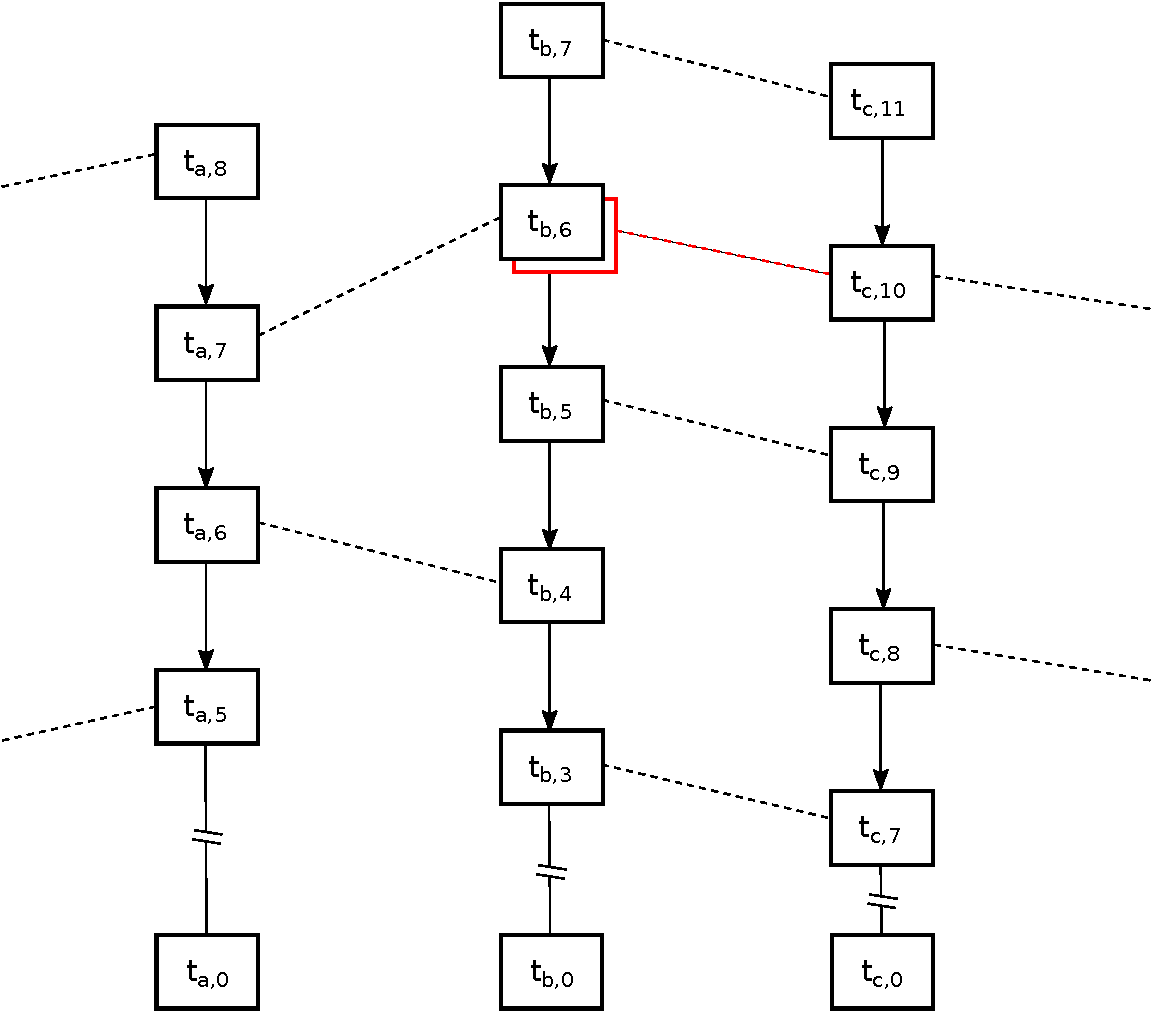
\includegraphics[width=0.9\textwidth]{trustchain-bad}
    \centering
    \caption{Every block is denoted by $t_{i,j}$, where $i$ is the node ID and $j$ is the sequence number of the block.
    Thus we have three nodes and three corresponding chains in this example.
    The arrows represent hash pointers and the dotted lines represent references.
    The blocks at the ends of one dotted line are pairs of each other.
    The red block after $t_{b, 5}$ indicate a fork.}
    \label{fig:trustchain-bad}
\end{figure}

If every node follows the rules of TrustChain and we only consider hash pointers,
then the chain effectively forms a singly linked list.
However, if a node violates the rules, then a \emph{fork} may happen.
That is, there may be more than one TX block with a hash pointer pointing back to the same block.
In \Cref{fig:trustchain-bad}, node $b$ (in the middle chain) created two TX blocks that both point to $t_{b, 5}$.
If this is a ledger system it can be seen as a double spend, where the currency accumulated up until $t_{b, 5}$ are spent twice.

\subsubsection*{Extended TrustChain}
We are now ready to explain the extended TrustChain, which we abbreviate to ETC.
In ETC, we introduce a new type of block, namely checkpoint (CP) block.
In contract to TX blocks, CP blocks do not store transactions or contain references.
They capture the state of the chain and the state of the whole system.
In particular, the state of the chain is captured with a hash pointer.
The state of the whole system is captured in the content of the CP block,
namely as a digest of the latest \emph{consensus result} which we explain in \Cref{sec:overview-cons}.
A visual representation is shown in \Cref{fig:trustchain-bad-cp}.

\begin{figure}
    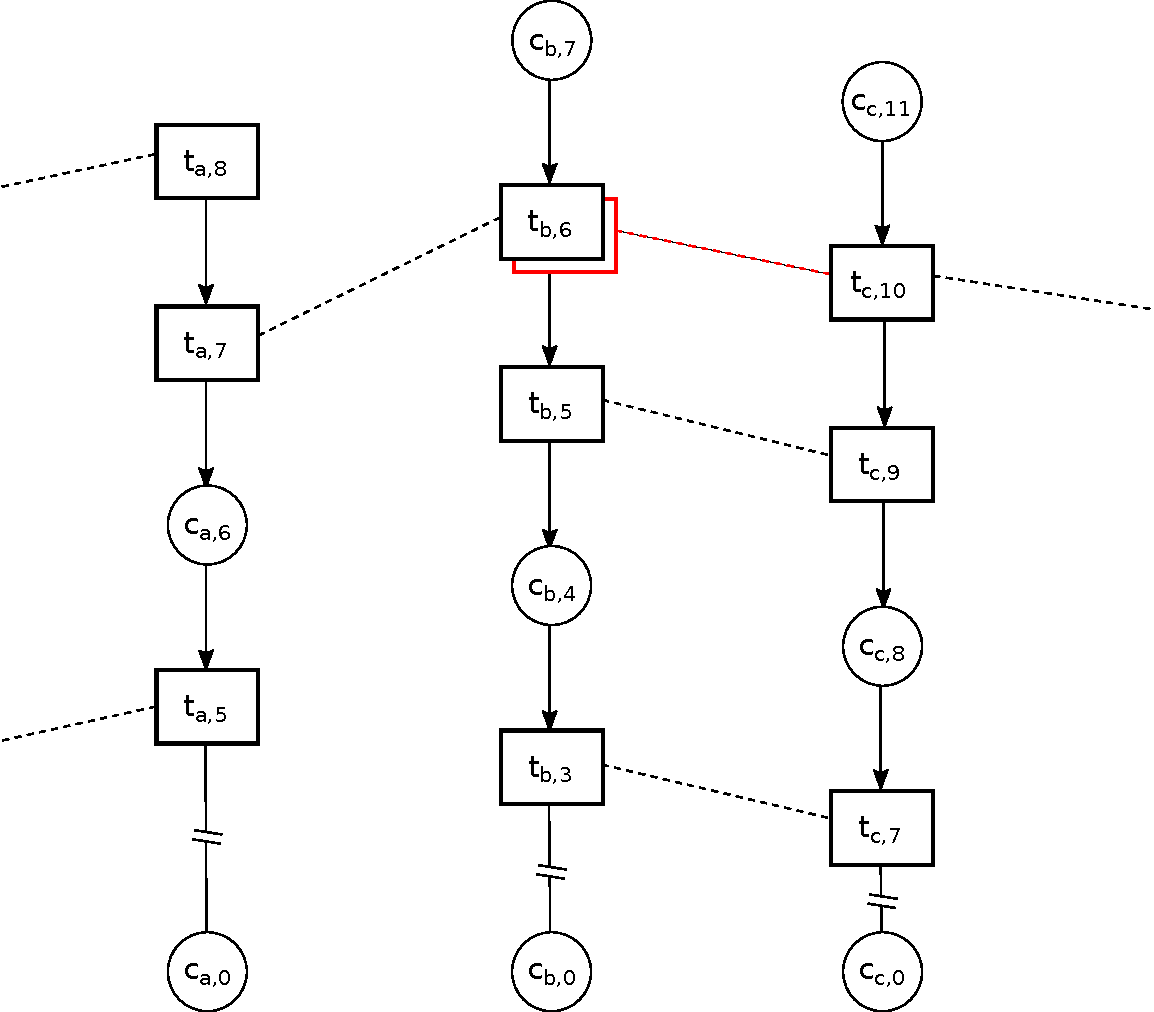
\includegraphics[width=0.9\textwidth]{trustchain-bad-cp}
    \centering
    \caption{The circles represent CP blocks,
    they also have hash pointers (arrow) but do not have references (dotted line).
    Note that the sequence number counter do not change, it is shared with TX blocks.}
    \label{fig:trustchain-bad-cp}
\end{figure}

\subsection{Consensus Protocol}\label{sec:overview-cons}
Before describing our consensus protocol, we take a brief detour to explain Byzantine consensus,
which is a fundamental building block of our consensus protocol.

\subsubsection*{Byzantine consensus}
Byzantine consensus is also known as \emph{atomic broadcast}.
Roughly speaking, atomic broadcast need to satisfy the following properties.
\begin{enumerate}
\item TODO
\end{enumerate}
TODO downsides (can't run with too many nodes) (high message complexity)
We stress that Byzantine consensus is not the same as Byzantine agreement or the Byzantine general's problem.
Byzantine agreement is TODO

The literature on Byzantine consensus and atomic broadcast is rich, some noteable ones include TODO.
Thus in the ETC consensus protocol, we assume there exist an "off-the-shelf" Byzantine consensus algorithm which we can use
(in our implementation we use HoneyBadgerBFT and motivate our choice in TODO).

In our case, every node do not propose some arbitrary data, but a set of CP blocks.
Thus the result of the consensus is the set union of all the legitimate proposals.

\subsubsection*{ETC consensus protocol} 
The consensus protocol runs continuously in rounds.
That is because a blockchain systems always need to reach consensus on new values, or CP blocks in our case.
This can be seen as running infinitly many rounds of some Byzantine consensus algorithm,
starting a new execution immediately after the previous one is completed.

As we mentioned earlier, the high message complexity prohibits us from running a Byzantine consensus algorithm on a large network.
Thus, for every round, we randomly select some node---called facilitators---to collect CP blocks,
and then use them as the proposal of the Byzantine consensus algorithm.
The facilitators are elected using a \emph{luck value}, which is computed using $H(\C_r || pk_i)$,
where $\C_r$ is the consensus result in round $r$ and $pk_i$ is the public key of $i$.
Intuitively, the election is guaranteed to be random 
because the output of a cryptographically secure hash function is unpredictable and $\C_r$ cannot be determined in advance.

A visual explaination can be found in \Cref{app:consensus-example},
it walks through the steps needed for a node to be selected as a facilitator.

\subsection{Transaction Protocol}
The TX protocol~\footnote{It is also known as True Halves, devised and implemented by Ewout Bongers.
See \url{https://github.com/Tribler/tribler/pull/2135} for more information.}
consist of two messages, \texttt{TX\_REQ} and \texttt{TX\_RESP}.
When a node  wishes to create a transaction,
it generates a TX block with the corresponding hash pointer, sequence number, counterparty and the transaction message itself.
It then sends a \texttt{TX\_REQ} message containing the TX block to the counterparty.
Upon receiving a TX block at the counterparty, it creates its own version of the TX block (the pair of the sender's TX block),
and sends it back to the sender in a \texttt{TX\_RESP} message.
At the end of the protocol, both parties should have both versions of the TX block.

\subsection{Validation Protocol}
The consensus and transaction protocol by themselves do not provide a mechanism to detect forks or other forms of tamperaing.
This is the goal of the validation protocol.

It also has two message---\texttt{VD\_REQ} and \texttt{VD\_RESP}.
When a node wishes to validate a transaction,
it sends a \texttt{VD\_REQ} with the sequence number $s$ to the party that created the TX block of the transaction.
Upon receiving a \text{VD\_REQ}, the node finds two \emph{agreed} CP blocks that surrounds the TX block and computes the \emph{fragment}.
An agreed CP block means that it has reached consensus.
A fragment of two CP blocks is a section of the chain where the beginning and the end are defined by those two CP blocks.
With the fragment, the node replies with a \texttt{VD\_RESP} message.
Upon receiving a \texttt{VD\_RESP}, the node checks that the fragment is created correctly.
Loosely, that means the agreed CP blocks have actually reached consensus,
the fragment has the correct hash pointers,
and TX block containing $s$ exists and is valid.


\subsection{Putting The Protocols Together}
The final protocol ($\Preal$) is essentially the concurrent composition of the three aforementioned protocols.
Our subprotocol design gives us the highly desireable non-blocking property.
In particular, we do not need to ``freeze'' the state of the chain for some communication to complete in order to create a block.
For instance, a node may start the consensus protocol, and while it is running, the node may still perform transactions.
By the time the consensus protocol is done, the new CP block is added to whatever the state that the chain is in.
It is not necessary to keep the chain immutable while the consensus protocol is running.

\section{Universally Composable Framework}
\label{sec:uc-intro}

In order to analyse the security of a system, a formal notion of security is required.
For instance, what does it mean if an encryption algorithm is secure?
One may say it is secure if the adversay cannot learn any information about the plaintext from the ciphertext.
But what if the adversay has some background information, for instance she may know it is English.
Do we then still say the encryption algorithm is secure?
Goldwasser and Micali introduced the notion of semantic security~\cite{goldwasser1982probabilistic}.
That is, imagine two worlds, a real world and an ideal world.
In the real world, the adversay is given the ciphertext,
and in the ideal world the adversay has nothing.
Then the encryption algorithm is semantically secure if the amount of information that the adversay can learn in the real world is just as much as the ideal world.
While our description is informal, the notion of security can be formally captured in this way.

Security sensitive distributed systems such as secure multi-party computation and blockchain systems also require a formal notion of security so that they can be analysed.
Fortunately, the idea from semantic security can also be applied in a distributed setting.
In an ideal world, we create an ideal functionality $\Fideal$ that performs all the computation on behalf of every node in the network.
The nodes act as dummies and only relay messages between $\Fideal$ and the environment.
Thus $\Fideal$ essentially becomes the specification of the distributed protocol.
If the execution of the real world protocol is indistinguishable from the ideal emulation in the presence of some adversay,
then the real world protocol is secure as per the ideal specification.
This is in essence the Universally Composable (UC) framework.

We use the UC framework not only because it suits our needs, 
it is also the only framework used in modelling blockchain systems to the best of our knowledge
~\cite{todo}TODO.
In the remainder of this section we give an overview of the UC framework.
A detailed treatment  can be found in~\cite{canetti2001universally}.

\subsection{Model of Computation}
The model of computation considered in the UC framework is the interactive Turing machine (ITM).
Specifically, an ITM is an extension of the Turing machine with externally writable tapes which are the following.
\begin{enumerate}
\item input tape---TODO
\item incoming communication tape---TODO
\item subroutine output tape---TODO
\end{enumerate}
ITM can be seen as a specification or an algorithm, a machine running an ITM is an ITM instance (ITI).
To communicate, an ITI can write on the externally writable tapes of other ITIs.
The writing ITI then pauses exeuction, the receiving ITI begins execution.
Consequently, only one ITI is running at any point in time.

\subsection{Simulation-based Security}
Simulation-based security, also known as ideal/real paradigm is a model for defining security.
The model consist of a set of , the environment $\E$, the adversay $\A$,
the protocol ITM $\Preal$ and zero or more ideal functionalities $\mathcal{F}_0, \mathcal{F}_1, \dots$.
The 
Other than the machines running the protocol under consideration, the model contains two extra entities,
the environment $\E$ and the adversary $\A$.
$\E$ can be seen as users of the protocol, it can only provide input and receive output from $\A$ and the protocol.

Control function TODO

\subsection{Universal Composability}

\section{Formal Specification}
\label{sec:formal-model}

The formal model follows the same structure as \ref{fig:todo}TODO.

\begin{framed}
\textbf{Protocol}\,$\Preal$

The ETC protocol. On initialisation do the following.
\begin{itemize}
\item Generate public and private key pair, $pk_i$ and $sk_i$.
\item Set personal chain $C := \{genesis\}$.
\item Set checkpoint buffer $\C' := \varnothing$.
\item Set the facilitators $F$ to the bootstrap nodes provided by $\E$.
\end{itemize}

Run the protocol as specified below after initialisation.
\begin{itemize}

\item Upon (\texttt{tx\_init}, $m$, $p$) from $\E$, 
    $C := C \cup \{new\_tx(m)\}$,
    send (\texttt{tx\_req}, latext TX in $C$) to $p$.
\item Upon (\texttt{tx\_req}, $m$) from $p \in \P$,
    $C := C \cup \{new\_tx(m)\}$,
    let $m'$ be the latest TX in $C$ and set $m$ to be the other half of $m'$,
    send (\texttt{tx\_resp}, $m'$) to $p$.
    Output the complete TX to $\E$.
\item Upon (\texttt{tx\_resp}, $m'$) from $p \in \P$,
    find the corresponding pair of $m'$ and name it $m$,
    add $m'$ as the other half of $m$.
    Output the complete TX to $\E$.

\item Upon (\texttt{vd\_init}, $s$) from $\E$,
    if the sequence number $s$ does not exist in $C$ or the block with $s$ does not have the other half then do nothing.
    Otherwise send (\texttt{vd\_req}, $s'$) to $p'$ where $s'$ is the sequence number of the other half and $p'$ is the counterparty.
\item Upon (\texttt{vd\_req}, $s'$) from $p \in \P$,
    if the sequence number $s'$ does not exist then do nothing.
    Otherwise send (\texttt{vd\_resp}, $agreed\_fragment(s')$) to $p$.
\item Upon (\texttt{vd\_resp}, $x$) from $p \in \P$,
    run $validate(x)$ and output result to $\E$.

\item Upon (\texttt{consensus}, $r$, $D$) from $\F_\text{BFT}$,
    TODO,
    send (\texttt{propose})

\item Upon (\texttt{checkpoint}, $c$) from $p \in \P$,


\end{itemize}

\end{framed}

\begin{framed}
\textbf{Functionality}\,$\F_\text{BFT}$

The ideal Byzantine consensus protocol, parameterised by...

\begin{itemize}
\item Upon (\texttt{propose}, $r$, $C$),
\item Upon (\texttt{fetch}),
\end{itemize}
\end{framed}

\subsection{Discussion}

\subsubsection{Global clock for synchronisation}
Where there is no Byzantine corruption, we conjecture that our protocol runs in the asynchronous setting.
However, security of many Byzantine consensus algorithms, especially the one we adopted---HoneyBadgerBFT,
fall apart when there is dynamic corruption.
In order to enforce that the corrupted machines do not change when running an instance of some Byzantine consensus algorithm,
we introduce synchrony.

We make use of a global clock... TODO

Dynamic corruption only between different clock ticks is enforced by the control function.

\subsubsection{Static corruption versus dynamic corruption}
A subtlety exists when modelling the type of corruption.
In dynamic corruption\footnote{In \cite{canetti2001universally}, dynamic corruption is termed Byzantine corruption.},
$\A$ take full control of a number of machines and also learns all of their states.
The states include private keys.
Thus, using the dynamic corruption model from \cite{canetti2001universally} we cannot guarantee security as
$\A$ can corrupt different machines over time and eventually learn all the private keys..

First is to use static corruption, where the corrupted machines are fixed.
While this circumvents our problem, it is a much weaker model.
Alternatively, we modify the aforementioned dynamic corruption model and weaken the adversary's abilities.
In particular, we introduce that forgetful adversary that only remembers the state of the currently corrupted nodes and forget the state of the recovered nodes.


\section{Protocol Extensions}
\label{sec:protocol-extensions}

